\documentclass[12pt]{report}
\usepackage[utf8]{inputenc}
\usepackage{amsmath}
\usepackage{amsfonts}
\usepackage{amssymb}
\usepackage{array}
\usepackage{color}
\usepackage{float}
\usepackage[margin=2.75cm]{geometry}
\usepackage{graphicx}
\usepackage{hyperref}
\usepackage{listings}
\usepackage{palatino}
\usepackage{parskip}
\usepackage{setspace}

\newcommand{\superscript}[1]{\ensuremath{^{\textrm{#1}}}}
\newcommand{\subscript}[1]{\ensuremath{_{\textrm{#1}}}}

%\newcommand{\th}[0]{\superscript{th}}
\newcommand{\st}[0]{\superscript{st}}
\newcommand{\nd}[0]{\superscript{nd}}
\newcommand{\rd}[0]{\superscript{rd}}

\newcommand{\amp}{{\fontfamily{ppl}\selectfont\emph\&}}

\lstset{numbers=left, basicstyle=\ttfamily, breaklines=true}

\renewcommand\chaptername{Section}

\begin{document}
	\onehalfspace
	
	\title{Sentiment Analysis, News \amp{} CAC40}
	\date{\today}
	\author{Alexis Daboville}
	
	\maketitle
	
	\begin{abstract}
		\ldots to be written \ldots
	\end{abstract}
	
	\pagenumbering{roman}
	\pagestyle{headings}
	\tableofcontents
	\listoffigures
	\listoftables
	
	\newpage
	
	\chapter*{Acknowledgements}
	
	\chapter{Introduction}
		% what? sentiment analysis? CAC?
		% why ?
		% how ?
		% hypothesis
	
	\chapter{Literature Review}
		
		In the past many authors suggested that the sentiments about a topic expressed in media may influence the ``actors'' of this topics. Examples of such studies include different topics like:
		
		\begin{itemize}
			\item Politics: sentiments may influence electors (e.g. K. Ahmad et al. \cite{ahmad11})
			\item Economy: sentiments may influence traders (e.g. P. Tetlock \cite{tetlock07})
		\end{itemize}
		
		These sentiments can come from several sources:
		\begin{itemize}
			\item News (e.g. K. Ahmad et al. \cite{ahmad11})
			\item Blogs (e.g. K. Ahmad et al. \cite{ahmad11})
			\item Social Networks (e.g. A. Pak et al. \cite{pak10})
		\end{itemize}
		
		In this study we will focus on sentiments expressed by economic newspapers, because we are interested in the impact of sentiments on stocks markets. In order to build an index of sentiments that varies over time and which not depends on the volume of news for a given day we compute the sentiments frequencies for each day. Of course we distinguish two main categories of sentiments: the positive ones and the negatives one.
		
		The studied market will be the CAC40. This is the major French stock index. It's composed by 40 of the most important French companies. Each company is pondered by a weight so the biggest company have more importance in the overall index. The most important companies being Total (oil), Sanofi (pharmaceuticals) and BNP Paribas (banking). The full list of the companies constituent the index can be found \href{http://en.wikipedia.org/wiki/CAC40}{here}. The method to compute index value can be found \href{http://www.euronext.com/fic/000/050/871/508718.pdf}{here}.
	
	\chapter{Methodology}
		\section{Getting the news}
		
			There was a few options to consider for getting news data. The first one was to know where to get the data, the second was how to get it.
			
			In 2009, Stéphane Kazmierczak \cite{kazmierczak08} did similar experiments and got his data by crawling the website Investir.fr\footnote{\url{http://www.investir.fr/}}. Investir.fr is a website about economy and stock markets. The problem is that there are two downsides using this approach:
			\begin{itemize}
				\item All the data comes from a single source.
				\item Currently most of economics news website have paid archives (which prevents me from crawling them).
			\end{itemize}
			
			The solution proposed by Khurshid Ahmad was to get the data from Lexis Nexis\footnote{\url{http://www.lexisnexis.com/en-us/home.page}}. Lexis Nexis is a platform which has numerous archives of newspapers (including French economic newspapers). Fortunately Trinity College has an agreement with them which allow Trinity students to use the service. Using this platform solved the two problems. In fact I was able to get data from multiple newspapers, and the Lexis Nexis website is ``crawlable''.
			
			However searching for archives for more than a few days is a tedious task. In consequence I developed a web crawler which browse Lexis Nexis automatically and download the data. Though, there was a few considerations to take into account. The first one was to crawl Lexis Nexis slowly to avoid to be ban from using the service. The second one was how to crawl the website. The first problem was easily solved, I decided to crawl no more than one month of data per day. So I needed roughly two months to get 63 months of data. The technical problem was more interesting. The first thing to consider is that I needed to be able to perform a lot of things with my robot: login, search for archives of each day by filling multiple forms, clicking on various links\ldots At first sight I though I would use Perl WWW::Mechanize\footnote{\url{http://search.cpan.org/dist/WWW-Mechanize/}} or Python Mechanize\footnote{\url{http://wwwsearch.sourceforge.net/mechanize/}}. Unfortunately none of them was able to handle the Javascript stuff (and Lexis Nexis heavily rely on the ability to execute Javascript). In consequence I quickly look on the Internet to find an alternative, and I found Watir\footnote{\url{http://watir.com/}}. Watir is described by Wikipedia\footnote{\url{http://en.wikipedia.org/wiki/Watir}} like that: ``\emph{Web Application Testing in Ruby (or Watir, [\ldots]) is a toolkit used to automate browser-based tests during web application development.}''. So even if it's primary designed for testing purposes we can use it to crawl a website. In fact Watir was the chosen solution because it was simple, and there was not any better alternative. Using Watir can be summed up in two steps:
			\begin{enumerate}
				\item Find the correct HTML\footnote{HyperText Markup Language.}/DOM\footnote{Document Object Model.} element.
				\item Set it to the right value and/or click it.
			\end{enumerate}
			
			For instance here's the method (part of the \lstinline!LexisNexisCrawler! class, in the file \lstinline!tools/lncrawler.rb!) that log the user in:
			
			\begin{lstlisting}[language=Ruby, basicstyle=]
def login(url, user='', pass='')
  # ask for login details
  # before going to login
  # page, so once it's filled user can "go away"
  # obviously if login details are 
  # provided to the method, does not ask
  while user.empty? or pass.empty?
    puts 'Username:'
    user = gets.chomp
    puts 'Password:'
    pass = gets.chomp
  end

  # goto login page
  @browser.goto url

  @browser.text_field(:name => 'user').set(user)
  @browser.text_field(:name => 'pass').set(pass)
  @browser.button(:name => 'Submit2').click
                                                                                                 
  # accept term & conditions
  @browser.link(:href => /submitterms\.do/).click

  # get the search link
  @searchUrl = @browser.link(:text => 'Search').href
end
			\end{lstlisting}
			
			Using the crawler developed with Watir I was able to fetch 560,000+ news. The time frame spans from January 1\st, 2004 to March 31\st, 2009. Also the data was collected from several French economic newspapers or websites:
			\begin{itemize}
				% + footnote with url to each website?
				\item L'Agefi quotidien
				\item Boursier.com
				\item Les \'Echos
				\item Les\'Echos.fr
				\item Le Figaro économie
				\item Investir.fr
				\item Le Parisien économie
				\item La Tribune
				\item LaTribune.fr
			\end{itemize}
			
		\section{Getting the CAC40 data}
		
			The CAC40 data was simply downloaded from Yahoo! Finance\footnote{\url{http://finance.yahoo.com/q/hp?s=^FCHI+Historical+Prices}} which provides all the data I needed in a handy  CSV file.
		
		\section{The dictionaries}
		
			To analyse the sentiments expressed in the news I also needed two dictionaries. The first one would contain the positive or negative words, and the second would contain the words related to economy.
			
			For the first dictionary, the idea used was to merge two things:
			\begin{itemize}
				\item The General Inquirer (GI) Dictionary\footnote{\url{http://www.wjh.harvard.edu/~inquirer/}} which is the reference dictionary for sentiment analysis. It classifies hundreds of words in several categories like strong or weak, positive or negative, active or passive\ldots Here I just needed the positive and negative categories.
				\item The most common words in economic news.
			\end{itemize}
			
			The GI dictionary was translated in French by Stéphane Kazmierczak, so I used it as a base.
			
			The most commons words were simply found using a little Python script. It just splitted all text in different words (in Python terms it means \lstinline!re.findall(r'\w+', text, re.UNICODE)!), and finally just use \lstinline!collections.Counter! and the \lstinline!.most_common()! method to find the most commons words.
			
			I merged the two dictionaries by hand because I wanted to add a few improvements over the Kazmierczak's one. The first thing was to only keep words that were often used in French. The second and more important improvement was to allow jokers at the end of the words. For instance instead of storing the words \emph{augmentation}, \emph{augmenter}, \emph{augmente} and so on I used a * as a joker and I just stored \emph{augment*}, so all words which have the prefix \emph{augment} are matched.
			
			The second dictionary was easy to build, I just translated (some of)\footnote{Only the ones that were translatable by a single word in French.} the economic words listed on InvestorWords.com\footnote{\url{http://www.investorwords.com/cgi-bin/bysubject.cgi?8}}.
			
			Then when I needed to lookup if a word is in one of the dictionary I used tries\footnote{Also known as prefix tree, see \url{http://en.wikipedia.org/wiki/Trie} for more informations.}, so the lookup was fast.
			
		\section{Processing the data}
		
			\emph{\color{red}I'm not sure I'll leave this here (3.4 \& 3.5): the definitions of sentiment frequencies/returns should probably go in the 1\st section\ldots}
		
			Once I had all the news the first thing to do was to reformat them. For example I had to remove useless metadata and normalize the dates (which were sometimes in French and sometimes in English\ldots). This work was done with a little Python script (\lstinline!tools/format.py!).
			
			Once it was done I was able to perform calculation over the corpus. For each day I computed the number of positive words, negative words and the total number of words, (see equations ~\ref{pwords}, ~\ref{nwords} and ~\ref{twords}).
			
			\begin{eqnarray}
			words(day) &=& \textrm{A set of all words in the news of day}\\
			\\			
			positive\_set &=& positive\_words\_set - economic\_words\_set\\
			positive\_words(day) &=& \sum_{w \textrm{ in } words(day)} (1\textrm{ if }w \textrm{ in } positive\_set \textrm{ otherwise } 0)\label{pwords}\\
			\\
			negative\_set &=& negative\ words\ set - economic\ words\ set\\
			negative\_words(day) &=& \sum_{w \textrm{ in } words(day)} (1\textrm{ if }w \textrm{ in } negative\_set \textrm{ otherwise } 0)\label{nwords}\\
			\\
			number\_of\_words(day) &=& length(words(day))\label{twords}
			\end{eqnarray}
			
			For better results, the function \lstinline!words(s)! splitted news using a regex. Then I used a function to remove all diacritical signs (so the words were kind of ``normalized'', for instance the word \emph{éléphant} is transformed to \emph{elephant}). This is done by the following Python code:
			
			\begin{lstlisting}[language=Python]
def normalize(w):
    """Convert an UTF-8 encoded string to a pure ASCII one.

    Also call lower on the word."""

    nfkd = unicodedata.normalize('NFKD', w)
    return ''.join(x for x in nfkd if unicodedata.category(x)[0] == 'L').lower()


_words_re = re.compile(r'\w+')
def words(s):
    """Returns all the words of a string."""

    return (normalize(w) for w in _words_re.findall(s))
    			\end{lstlisting}

				The final step of processing the data was to merge the CSV produced by the script which count the words (\lstinline!tools/count.py!) and the CAC40 data into another CSV file. This was done by another Python script (\lstinline!tools/merge.py!). During this step I also computed the frequencies of positive and negative words (equations ~\ref{pfreq} and ~\ref{nfreq}).
			
			\begin{eqnarray}
				positive\_freq(day) &=& \frac{length(positive\_words(day))}{number\_of\_words(day)}\label{pfreq}\\
				negative\_freq(day) &=& \frac{length(negative\_words(day))}{number\_of\_words(day)}\label{nfreq}
			\end{eqnarray}
			
			Usually the sentiment frequencies are defined as the average of the sentiment frequency of each news for a given day. I decided to do it differently because doing it this way gives \emph{less weight} to short stories.
			
		\section{Analysis of the data}
			
			The analysis of the data was done with LibreOffice Calc\footnote{\url{http://www.libreoffice.org/features/calc/}} which is a free and open source alternative to Microsoft Excel\footnote{\url{http://office.microsoft.com/en-us/excel/}}. To use it I just needed to import the  CSV file produced at the merge step. Then I was able to use the common functions like: \lstinline!AVERAGE!, \lstinline!STDEV!, \lstinline!PEARSON!, etc).
			
			Using LibreOffice Calc I performed several computations. I began by plotting the $positive\_freq(day)$, $negative\_freq(day)$, $close\_cac40(day)$ and $volume\_cac40(day)$. I also computed the mean and the standard deviation of each of these variable. Then I computed their daily logarithmic return. The logarithmic return is defined as equation ~\ref{return} (Wikipedia\footnote{\url{http://en.wikipedia.org/wiki/Rate_of_return\#Logarithmic_or_continuously_compounded_return}}).
			
			\begin{eqnarray}
				return = \ln\frac{V_f}{V_i}\label{return}
			\end{eqnarray}
			
			Where $V_f$ is the final value investment and $V_i$ the initial value of investment. In order to compute daily returns we use equations ~\ref{preturn}, ~\ref{nreturn}, ~\ref{creturn} and ~\ref{vreturn}.
			
			\begin{eqnarray}
				positive\_return(day) &=& \ln\left(\frac{positive\_freq(day)}{positive\_freq(previous\_day(day))}\right)\label{preturn}\\
				negative\_return(day) &=& \ln\left(\frac{negative\_freq(day)}{negative\_freq(previous\_day(day))}\right)\label{nreturn}\\
				close\_return(day) &=& \ln\left(\frac{close\_freq(day)}{close\_freq(previous\_day(day))}\right)\label{creturn}\\
				volume\_return(day) &=& \ln\left(\frac{volume\_freq(day)}{volume\_freq(previous\_day(day))}\right)\label{vreturn}
			\end{eqnarray}
			
			Finally I computed the 1 month volatility of the same variables which is the standard deviation of their returns over a 30 day period.
			
	\chapter{Experiments and Evaluation}
		\section{Graph analysis}
		
			To get an insight of the data the first thing I did was to plot the data against time (see figures ~\ref{cac}, ~\ref{pos}, ~\ref{neg} and ~\ref{posdivneg}). It worth to be noted that the plots of returns and volatility does not show anything interesting --except that the magnitude of both returns and volatility of the CAC40 is higher since the end of 2008-- that's why they are not included here.

			\begin{figure}[h!]
				\caption{CAC40 close over time\label{cac}}
				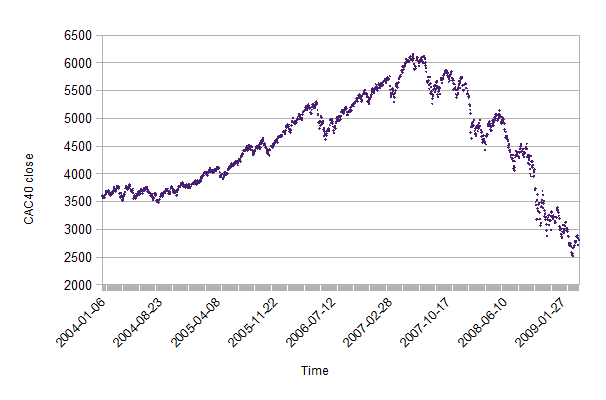
\includegraphics{plots/time/cac.png}
			\end{figure}

			\begin{figure}[h!]
				\caption{Positive sentiments frequency over time\label{pos}}
				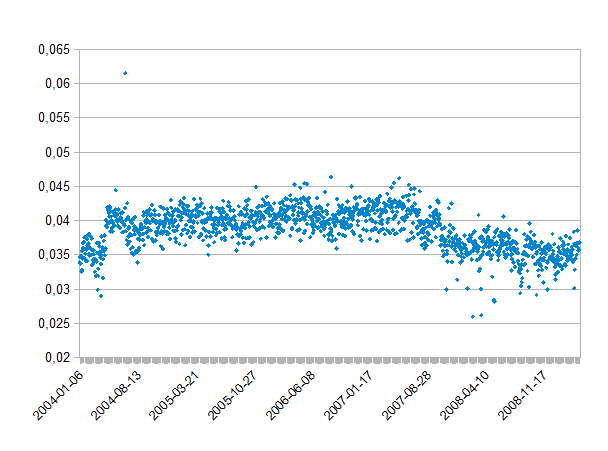
\includegraphics{plots/time/pos.png}
			\end{figure}
	
			\begin{figure}[h!]
				\caption{Negative sentiments frequency over time\label{neg}}
				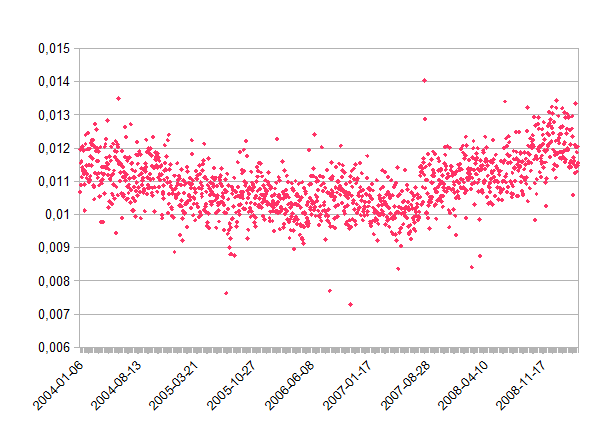
\includegraphics{plots/time/neg.png}
			\end{figure}
			
			\begin{figure}[h!]
				\caption{$\dfrac{positive\ sentiments\ frequency}{negative\ sentiments\ frequency}$ over time\label{posdivneg}}
				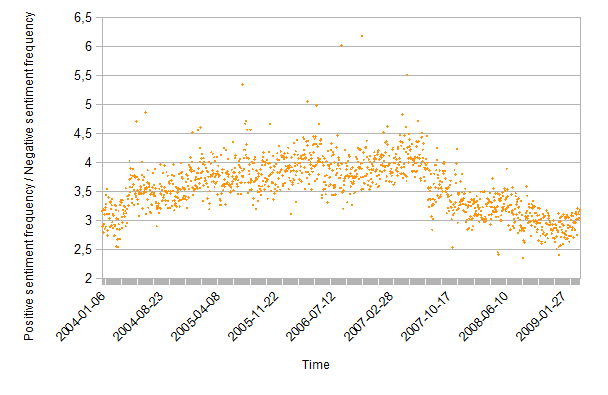
\includegraphics{plots/time/posdivneg.png}
			\end{figure}
			
			The first thing to notice is that all the graph can be divided in the same periods:
			\begin{itemize}
				\item Before mid-2007
				\item Mid-2007
				\item After mid-2007
			\end{itemize}

			 We can sum up the trends in a table (see Table ~\ref{trends}). It's now easier to compare the time series with each other:
			 \begin{itemize}
			 	\item The level of positive sentiments is higher when the CAC40 goes up and lower when it goes down.
			 	\item The level of negative sentiments seems to be the opposite of the CAC40 movements.
			 	\item $\dfrac{Positive\ sentiments\ frequency}{Negative\ sentiments\ frequency}$ roughly follows the same directions than the CAC40.
			 \end{itemize}

			\begin{center}
			\begin{table}
			\begin{tabular}{|c | c | c | c|}
				\hline
				& Before mid-2007 & Mid-2007 & After mid-2007\\
				\hline
				CAC40 close & $\nearrow$ & $\rightarrow$ $\searrow$ & $\searrow$\\
				\hline
				Positive sentiments frequency & $\rightarrow$ & $\searrow$ & $\rightarrow$\\
				\hline
				Negative sentiments frequency & $\searrow$ & $\rightarrow$ & $\nearrow$\\
				\hline
				$\dfrac{Positive\ sentiments\ frequency}{Negative\ sentiments\ frequency}$ & $\nearrow$ $\rightarrow$ & $\searrow$ & $\searrow$\\
				\hline
			\end{tabular}
			\caption{CAC40 and sentiments trends\label{trends}}
			\end{table}
			\end{center}
			
			This clearly shows that the sentiments and the CAC40 follows some trends during \textbf{the same periods} and \textbf{may be somewhat related}. This is leaves us two questions: does CAC40 trends follows sentiments trends (or the opposite)? Can we draw the same conclusion on a daily basis (instead of a four years time frame)?
			
			Another interesting thing to visualize is the distribution of return (see figures ~\ref{dist_cac}, ~\ref{dist_vol}, ~\ref{dist_sentiments}). Even if it proves nothing the fact that all distributions are the same shows that our hypothesis remains plausible. If the distributions have been totally different, the hypothesis would have been wrong.

			\begin{figure}[H]
				\caption{Distribution of the CAC40 close returns\label{dist_cac}}
				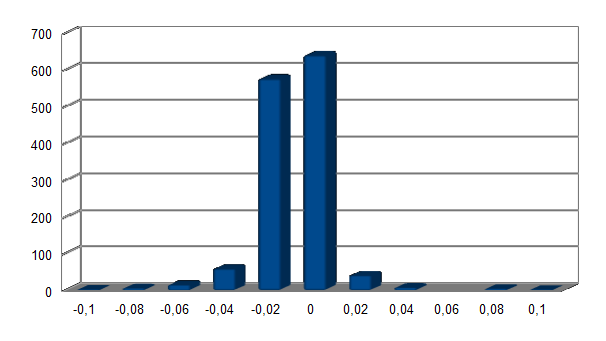
\includegraphics{plots/dists/close_return.png}
			\end{figure}

			\begin{figure}[H]
				\caption{Distribution of the CAC40 volume returns\label{dist_vol}}
				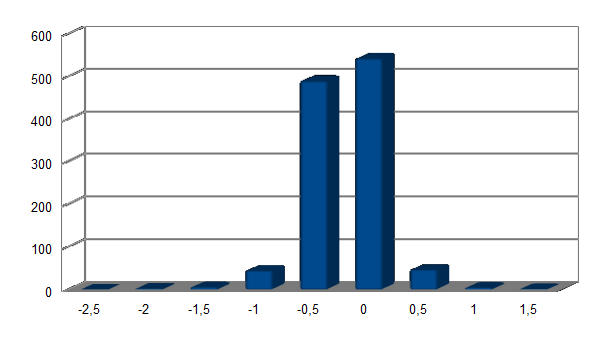
\includegraphics{plots/dists/volume_return.png}
			\end{figure}

			\begin{figure}[H]
				\caption{Distribution of the sentiments returns\label{dist_sentiments}}
				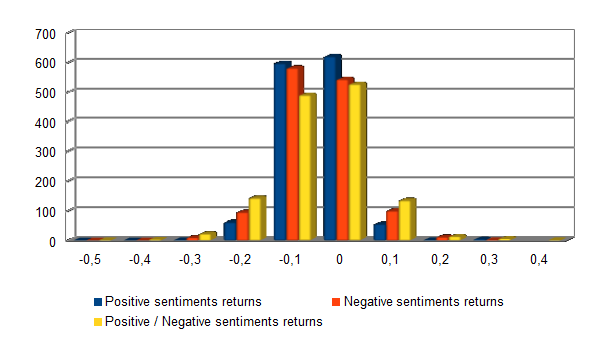
\includegraphics{plots/dists/pos_neg_posneg_returns_dist.png}
			\end{figure}
			
		\section{Correlation between news and the CAC}

			The primary goal of this project was to show if there's a correlation between sentiments expressed in economic news and the daily changes of the CAC40. It's possible to search a correlation between the returns or the volatily of the CAC/the sentiments.
			
			To do this I used the Pearson correlation\footnote{\url{http://en.wikipedia.org/wiki/Pearson_product-moment_correlation_coefficient}}. Pearson correlation is a mathematical tool which try to show if there's a correlation between two datasets. It gives us a \emph{correlation coefficient} in the range $[-1, 1]$. If the value of $|correlation\ coefficient|$ is close to 1 this means that it exists a strong correlation between the two datasets, a value close to 0 means that there's no correlation.
			
			Correlation coefficients between returns of sentiments, CAC40 close and CAC40 volume were calculated. I computed them on the same day or with an interval of one day (to see if news forecasts the CAC40 or the inverse). The results are shown in the table ~\ref{pearson_cac} and ~\ref{pearson_volume}. We can see that all the coefficients are within the interval $[-0.1, 0.1]$ which means that we cannot show that there's a correlation between the returns of sentiments and the returns of the CAC40 or the returns of the CAC40 volume.
			
			\begin{table}
			\begin{tabular}{|c | c | c | c|}
				\hline
				Sentiments date and CAC40 date & Positive sentiments & Negative sentiments & $\dfrac{Positive}{Negative}$\\
				\hline
				previous(day) and day & -0.0280 & -0.0583 & 0.0292\\
				\hline
				day and day & 0.0450 & -0.0764 & 0.0956\\
				\hline
				next(day) and day & 0.0491 & 0.0305 & 0.0089\\
				\hline
			\end{tabular}
			
			\caption{Pearson correlation between sentiments returns and CAC40 returns.\label{pearson_cac}}
			\end{table}

			\begin{table}
			\begin{tabular}{|c | c | c | c|}
				\hline
				Sentiments date and CAC40 date & Positive sentiments & Negative sentiments & $\dfrac{Positive}{Negative}$\\
				\hline
				previous(day) and day & -0.0655 & 0.0537 & -0.0899\\
				\hline
				day and day & -0.0201 & -0.0681 & 0.0433\\
				\hline
				next(day) and day & 0.0936 & 0.0473 & 0.0247\\
				\hline
			\end{tabular}
			
			\caption{Pearson correlation between sentiments returns and CAC40 volume returns.\label{pearson_volume}}
			\end{table}

		To be complete I also computed other correlations about volatility:
			\begin{itemize}
				\item Between sentiments and CAC40 close, table ~\ref{pearson_vol_cac}.
				\item Between sentiments and CAC40 volume, table ~\ref{pearson_vol_vol}.
			\end{itemize}
			However all the correlation coefficients are in the interval $[-0.21, 0.32]$. This is better than the returns correlations, but this is still low.

			\begin{table}
			\begin{center}
			\begin{tabular}{|c | c | c|}
				\hline
				Positive sentiments & Negative sentiments & $\dfrac{Positive}{Negative}$\\
				\hline
				0.1240 & -0.1029 & -0.3180\\
				\hline
			\end{tabular}
			\end{center}
			
			\caption{Pearson correlation between sentiments volatility and CAC40 volatility (over 30 days).\label{pearson_vol_cac}}
			\end{table}

			\begin{table}
			\begin{center}
			\begin{tabular}{|c | c | c|}
				\hline
				Positive sentiments & Negative sentiments & $\dfrac{Positive}{Negative}$\\
				\hline
				-0.2061 & 0.0846 & 0.0567\\
				\hline
			\end{tabular}
			\end{center}
			
			\caption{Pearson correlation between sentiments volatility and CAC40 volume volatility (over 30 days).\label{pearson_vol_vol}}
			\end{table}

		\section{Toward a better hypothesis}

		If we look at the CAC40 close data we can see that two consecutive close are highly correlated (the correlation coefficient is higher than 0.99). We can also see that this remains true for closes separated by a few days. So we may try another hypothesis, see equation ~\ref{hypo_cac}.

			\begin{eqnarray}
				cac40\_close(t) = \alpha_0 + \sum_{i = 1}^{n}\left(\alpha_i\times{}cac40\_close(t - i)\right) + \varepsilon(t)\label{hypo_cac}
			\end{eqnarray}

			For some small $n$, say 7. The interesting part is the error term $\varepsilon(t)$. It's a small variation and we make the hypothesis that its value is influenced by sentiments.

			To find the $\alpha_i$ I used an autoregressive model\footnote{I used a Python module by Ernesto Adorio which can be found \href{http://adorio-research.org/wordpress/?p=4551}{here}.}, ``trained'' over 90\% of the data. Then I computed the error term produced by the model on the remaining 10\% of the data, see equation ~\ref{hypo_epsilon}.

			\begin{eqnarray}
				\varepsilon(t) = cac40\_close(t) - \alpha_0 - \sum_{i = 1}^{7} \left(\alpha_i\times{}cac40\_close(t - i)\right)\label{hypo_epsilon}
			\end{eqnarray}

			Finally to test the validity of the hypothesis I computed various correlations between sentiments and $\varepsilon(t)$. The results can be seen in the table ~\ref{pearson_cac_ar}. Again the correlations coefficients are low (in the interval $[-0.1, 0.3]$) \emph{but} they are higher than the direct correlation between returns. So even if the correlation is far from perfect it looks like this hypothesis is better. Obviously they are numerous factors distincts from sentiments which occurs in the value of $\varepsilon(t)$, that's why the correlation is low.

			\begin{table}
			\begin{tabular}{|c | c | c | c|}
				\hline
				Sentiments date and CAC40 date & Positive sentiments & Negative sentiments & $\dfrac{Positive}{Negative}$\\
				\hline
				previous(day) and day & -0.06 & 0.17 & -0.10\\
				\hline
				day and day & 0.17 & -0.05 & 0.17\\
				\hline
				next(day) and day & -0.08 & 0.27 & 0.17\\
				\hline
			\end{tabular}

			\caption{Pearson correlation between sentiments and $\varepsilon(t)$\label{pearson_cac_ar}}
			\end{table}

			It's also possible to apply the same analysis with the CAC40 volume, where the formula is nearly the same, see equation ~\ref{hypo_vol} (the only change is $\alpha_i \rightarrow \alpha_{v_i}$ and $\varepsilon(t) \rightarrow \varepsilon_v(t)$ to avoid confusion).

			\begin{eqnarray}
				cac40\_volume(t) = \alpha_{v_0} + \sum_{i = 1}^{7}\left(\alpha_{v_i}\times{}cac40\_volume(t - i)\right) + \varepsilon_v(t)\label{hypo_vol}
			\end{eqnarray}

			I applied the same process to find the $\alpha_{v_i}$ and then I computed the correlations coefficient between sentiments and $\varepsilon_v(t)$ (see table ~\ref{pearson_cac_vol_ar}). We can draw the same conclusions as for the close data: the coefficients are still low (in $[-0.24, 0.30]$) \emph{but} they are higher than the simple correlation between returns.

			\begin{table}
			\begin{tabular}{|c | c | c | c|}
				\hline
				Sentiments date and CAC40 date & Positive sentiments & Negative sentiments & $\dfrac{Positive}{Negative}$\\
				\hline
				previous(day) and day & -0.13 & 0.16 & -0.24\\
				\hline
				day and day & 0.13 & 0.30 & -0.16\\
				\hline
				next(day) and day & 0.05 & 0.14 & -0.09\\
				\hline
			\end{tabular}

			\caption{Pearson correlation between sentiments and $\varepsilon_v(t)$\label{pearson_cac_vol_ar}}
			\end{table}

	\chapter{Afterword}
		% conclusion
		% results?
		% future work
		% - nn?
		% - 7? try with other value in [1,15]
		% - non linear correlation
		% - nltk
		% - global world? only french news? maybe not
		
	\bibliographystyle{plain}
	\bibliography{biblio}		
\end{document}
